\chapter{Security Concepts}

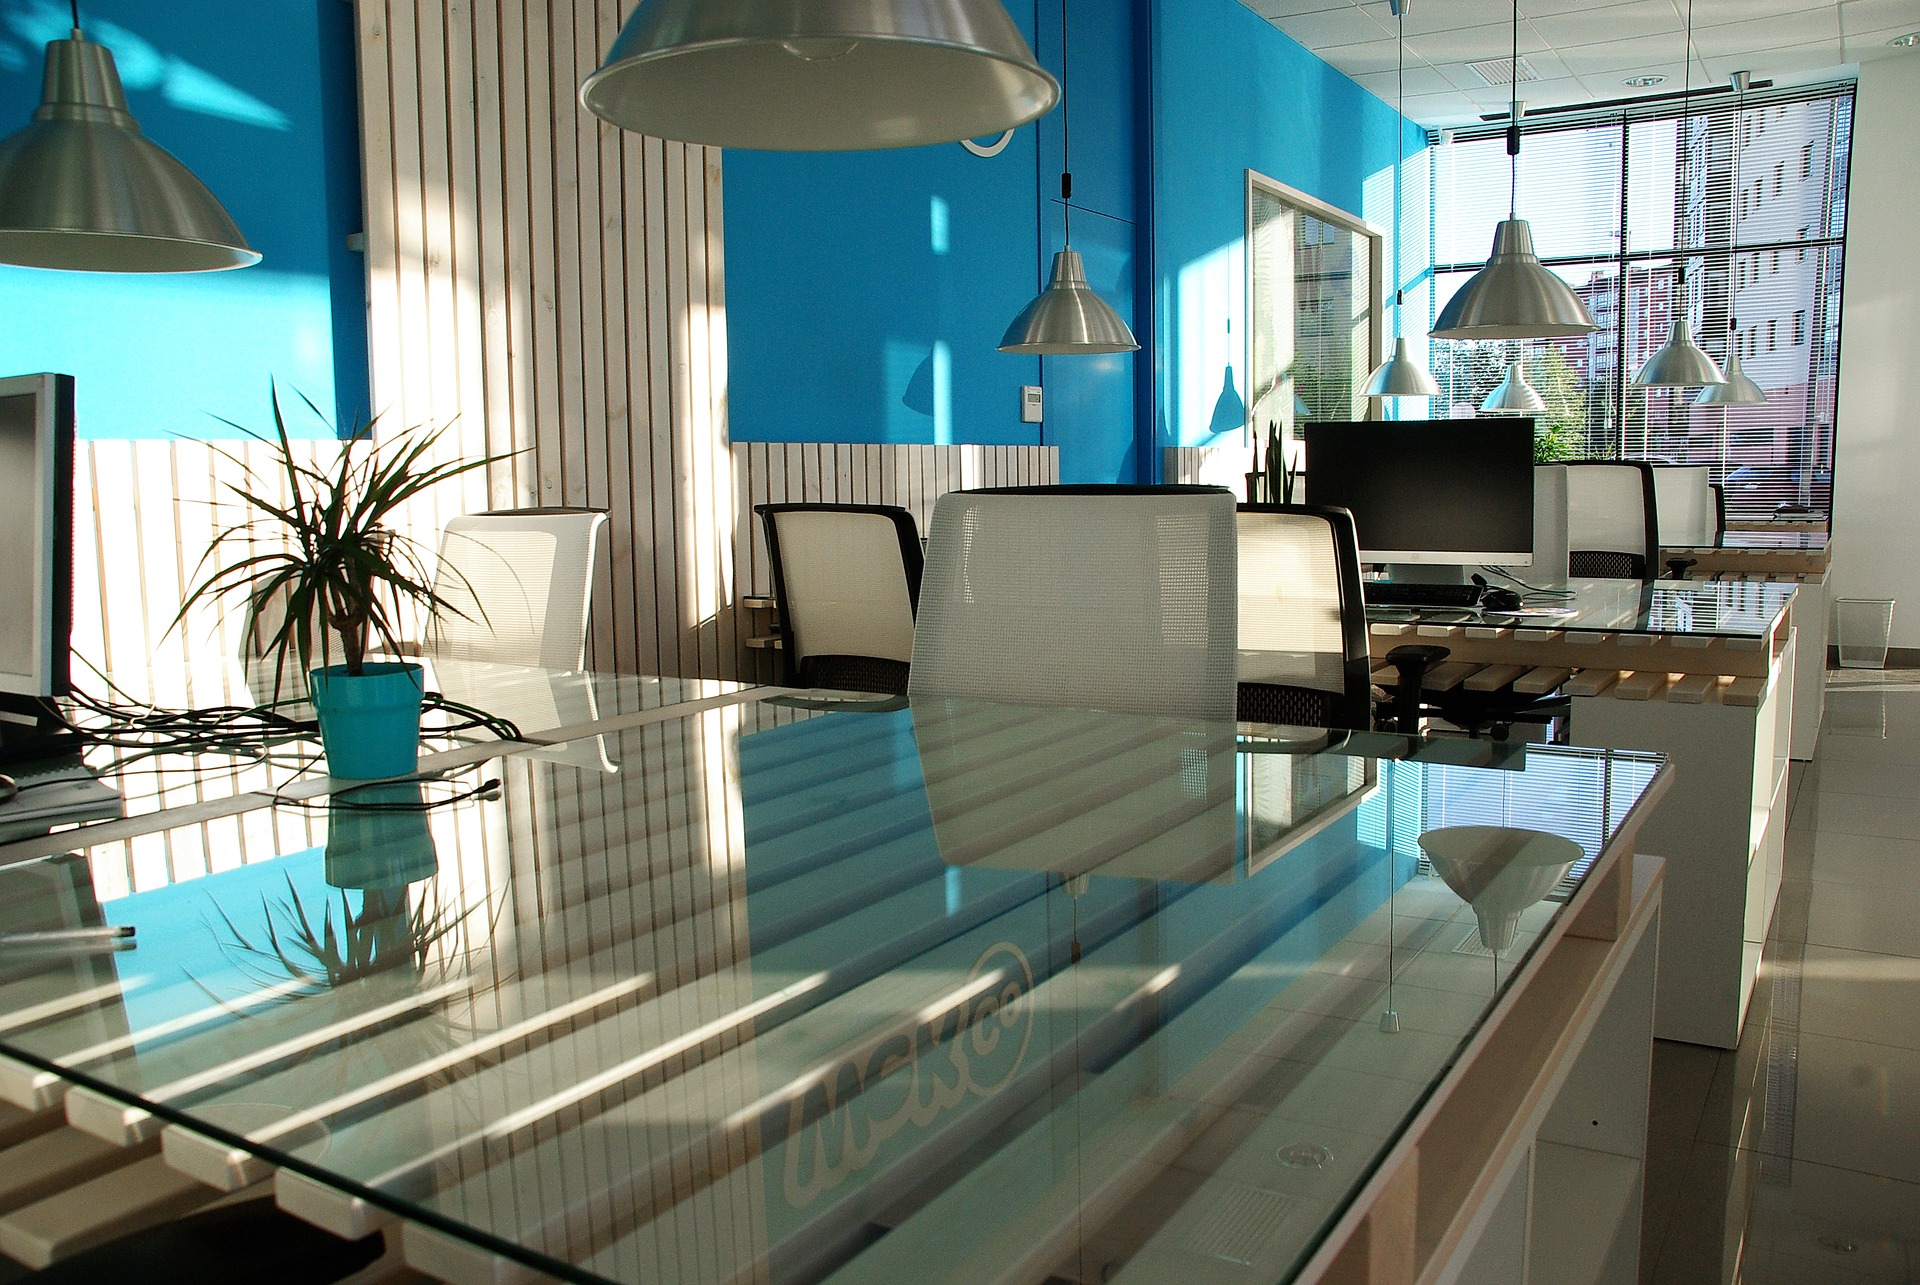
\includegraphics[scale=0.85]{images/office-space-1744803_1920.jpg}

\justifying
Shifting gears a bit so that security is top of mind, there are some ideas we can explore that will help ue meet our goal of 
putting out the most secure product possible.

\section{Security Mindedness}

\justifying
This is the concept that security should be a part of all the things.

\section{Shifting Left}

\justifying
We now have a mental picture of how software will flow through our three environments, from
Development, to Test, and finally into Production where it is accessible to the widest
base of consumers. Integration of best security practices into this flow, as early and as often
as possible, is highly desirable.

\justifying
Imagine our software life cycle occurring along a temporal axis, t. Intentionally moving security to the
left on this axis (lower values of t) is known as ``Shifting Left''\index{Shift Left} as seen
in figure \ref{shift}.

\begin{figure}
	\centering
	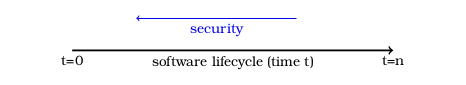
\includegraphics{images/shift_left.png}
	\caption{Shifting Left}
	\label{shift}
\end{figure}

\section{Zero Trust}

\justifying
Starting from the assumption that all the computers and networks are inherently unsafe and/or already compromised, the
Zero Trust model gives organizations a way of thinking when establishing a security posture.\cite{zerotrust} This premise,
while rather simple from the conceptual standpoint, can be anything but when it comes to application. The difficulties in
scaling this mindset up for larger organizations can quickly become anything but simple.

